\chapter{Introduction}
\section{Motivation}

Imagine you are sitting in your office, dozing off, ready to sleep. As soon as you fall asleep, someone pulls a prank on you and takes you to a different room. Shortly afterwards you wake up confused not knowing where you are. What would you do in this situation? You would probably look around to check if you are still inside the building. Then you would try to pinpoint your location based on what you see inside the room. If that was not enough information you could go outside and start exploring the environment. If you have been here before, you would probably be able to recognize some similarities and find out where you are. Then you could just go back to your office, and continue where you left off. It might seem to be an intuitive task for you, however robots cannot solve it quite as easily.

\section{Objectives}

In this work we tackle the kidnapping problem on robots. The first step is to detect whether a kidnapping situation occurred and the second step is to relocalize itself. Detection can be done by determining whether some information from the sensors is missing or whether the perceived environment does not match the expected one. Recovery can be done by gathering  information while exploring the surroundings. If any known features are found, they will be matched with the robot's database. Successful matching means that the robot can use the results to estimate its position in the environment. Otherwise, the exploration continues.

\chapter{Fundamentals}
\section{ROS -- the Robot Operating System}
ROS is an open-source framework for robot software that was initially developed at Willow Garage in Palo Alto after ideas for it originated in the \textsc{Stair} and Personal Robotics research projects at Stanford University in 2007. 

ROS aims to simplify development of complex robotic systems by introducing a vast ensemble of tools and packages for solving common robotics tasks. Among others these include typical features of an operating system such as hardware abstractions, inter-process communication, network communication, package management as well as compilers and libraries for supported languages. As of now ROS has been written for C++, Python and Lisp.

\subsection{Network Communication}
A ROS system typically consists of multiple interacting programs called \textit{nodes} and the \textit{ROS Master} that registers them and handles communication.

Nodes can communicate asynchronously by using the \textit{Publisher-Subscriber} pattern: To send data, a node can publish to self-defined \textit{topics} and listen on other topics. Each topic is described by the type of \textit{messages} that are published on it. The description is a \texttt{csv}-similar \texttt{.msg}-file containing data types and an optional timestamp.
A topic can be published to and listened on by many nodes. Consequently participants are agnostic about the identity of publishers.
\\\\
Alternatively synchronous communication is realized with \textit{Services} that are defined by message types for service requests and service replies. A node can act as a service and registers at the ROS Master with its name. Then other nodes can contact it by querying its address from the Master. Interaction with it runs over a newly established TCP/IP- connection and is similar to a remote procedure call.

\subsection{Monitoring}
ROS also provides means for monitoring the running system. For example nodes can publish to the \texttt{rosout}-topic for logging purposes.

Several Command line tools display information on loaded entities, e.g. \textit{rosnode} shows information about active nodes such as its publications and subscriptions, supports pinging them, manually killing nodes etc. Similarly \texttt{rostopic}, \texttt{rosservice} and \texttt{rosmsg} provide information and commands on the respective subjects.

Alternatively qt-based GUI tools can be used. For example \texttt{rqt\_deps} generates a pdf with all used ROS dependencies. \texttt{rqt\_graph} displays a graph of nodes and topics.

One of the most powerful tool is probably \texttt{rviz}: A 3D visualizer that continuously displays information read from topics such as robot positions, point clouds, odometry data, polygons, maps and many more. If available displays are not satisfactory, the user can also use generic markers to visualize arbitrary data.

\section{MCA2 -- Modular Controller Architecture Version 2}
MCA2 is a C++ robotics framework developed at the FZI in Karlsruhe between 1998 and 2012. It is organized in groups of multiple modules with a standardized set of 5 interfaces: 
\begin{itemize}
\item Sensor input
\item Sensor output
\item Controller input
\item Controller output
\item Internal parameters and variables
\end{itemize}

The input and output interfaces serve as communication points to other modules. They are data vectors of varying dimensions between which are data manipulating \texttt{sense()} and \texttt{control()} edges. E.g. sensor input can be passed into a module which alters the data and passes it on to the next module. The fifth module is able to alter the modules internal parameters at runtime.

Module groups are arranged in hierarchical order. To the outside they appear like any other module, but each call to the group's \texttt{control()} or \texttt{sense()} function initiates a cascade of calls to the contained modules in hierarchical order.

An MCA part consists of multiple groups and modules. It executes them in a loop and can also run them in so-called \texttt{ThreadControllers}.

\section{Kinect}
The Kinect is a 3D camera sensor developed by Microsoft for the Xbox video game console. In 2011 Microsoft released the Kinect for Windows SDK, one year later it released the Kinect robotics SDK.

With its ability to recognize motion and distances, it is very well suited to assist basic robot movement and orientation tasks: obstacle avoidance, environment mapping, distance detection, object tracking etc.

In this work we primarily rely on the Kinect's object tracking abilities.
  
\section{Laser Scanner}
3D laser scanner use narrow laser-beam to scan their environment and allow almost continuous scanning - regardless of whether objects are moving or not. As a result, 3D laser scanner gets a set of points which represent the direction and distance of objects in around. Sick LMS100 (shown in Figure \ref{Laser}) has the scanning angle of  270$^\circ$ and has high detection capability.

We can get the output from laser scanner in ROS with sensor\_masgs/LaserScan message. The message is made up of several parts, including header, ranges, and other information of laser scaner. The start and end angle of the scan, angular distance between measurements, time between measurements, minimum and minimum range value are stored in this message. Most important information we need is the angle of each hit and its distance (range) from the scanner.

\begin{figure}[thpb]
      \centering
      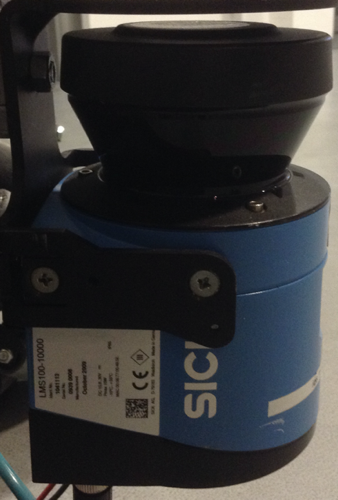
\includegraphics[width=0.5\textwidth]{graphics/Laserscanner.png}
      %\includegraphics[scale=1.0]{figurefile}
      \caption{Sick LMS100}
      \label{Laser}
   \end{figure}
\section{ASAP (Advanced Shared Autonomy Platform)}
The ASAP (shown in Figure \ref{ASAP}), short for Advanced Shared Autonomy Platform, is a mobile robotic platform based on two Segway RMP-50 Omni platforms. The Platform is mounted with four omnidirectional plastic rollers, so that the Segway can free move in all directions (shown in Figure \ref{Omni}). In addition, this ASAP includes some sensors, on-board comoputer, software system. For sensor, there are Two Sick LMS100 laser scanners and a Kinect on top. The embeded computer is Esperia, which has 4G ram, 64G SSD, core i7 M620 CPU and can be connected through WLAN address 141.21.13.215. Ubuntu 14.04 Trusty, ROS Indigo, MCA2 are three main software systems in this ASAP.

\begin{figure}[thpb]
      \centering
      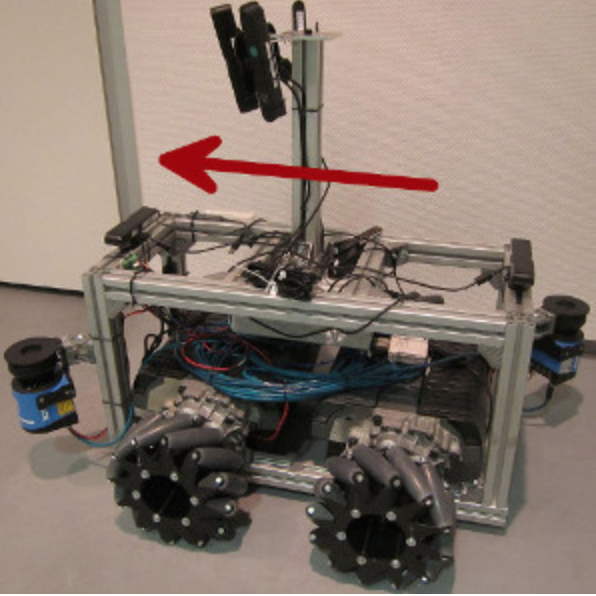
\includegraphics[width=0.5\textwidth]{graphics/ASAP.png}
      %\includegraphics[scale=1.0]{figurefile}
      \caption{The structer of Advanced Shared Autonomy Platform, and red arrow shows the forward direction of the platform, which is the same as the X axes in ROS.}
      \label{ASAP}
   \end{figure}

\begin{figure}[thpb]
      \centering
      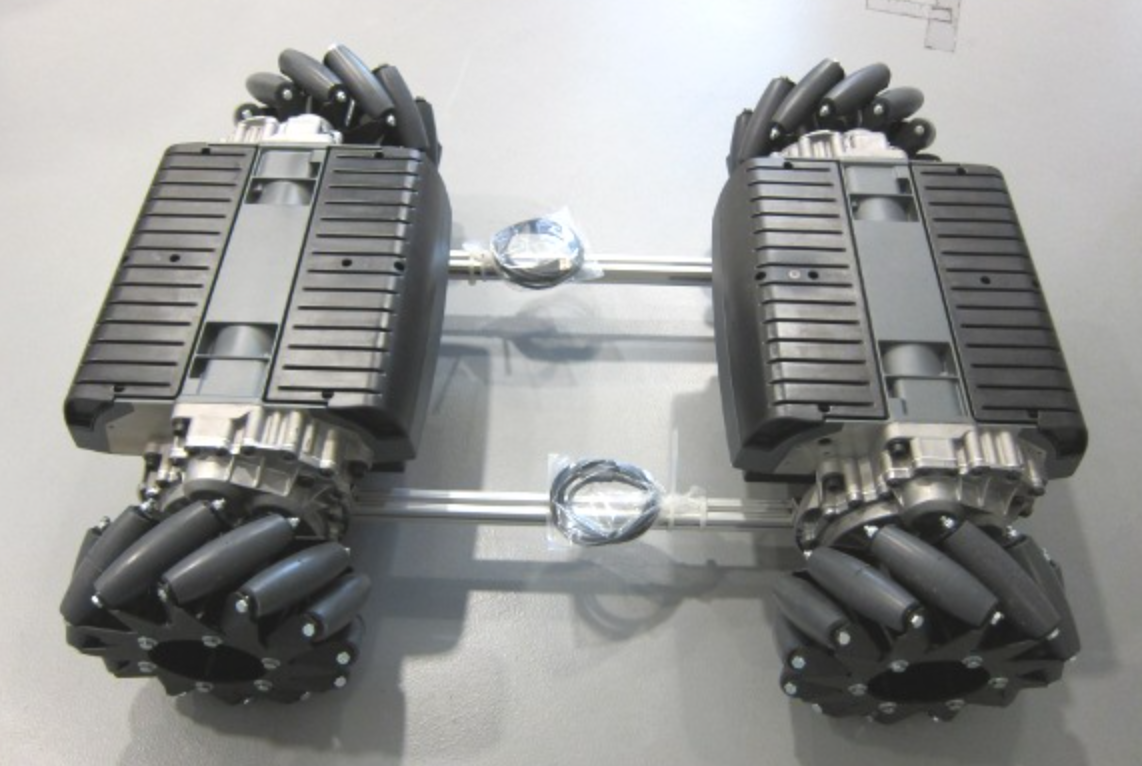
\includegraphics[width=0.5\textwidth]{graphics/SegwayPlattform.png}
      %\includegraphics[scale=1.0]{figurefile}
      \caption{The Segway RMP-50 Omni Plattform includes Mecanum-Rad and Batterie.}
      \label{Omni}
   \end{figure}

\section{Kalman Filter}
Many problems in the domain of artificial intelligence require the prediction of future states by evaluating measurements. Around the 1960s Peter Swerling, Rudolf E. Kálmán, Thorvald N. Thiele and Richard Bucy described an algorithm for this purpose. It is now known as the \textit{Kalman filter}.

In the field of robotics Kalman filters can be utilized to predict future poses for a moving robot by continuously combining measurements from various sources. A Kalman filter is therefore a sensor fusion algorithm. Common sensors are
 
\begin{itemize}
\item motion sensors that estimate position change over time (odometry),
\item laser scanners that scan the environment,
\item cameras that track predefined markers. 
\end{itemize}

By combining the last estimation and the current sensor outputs a new estimation for the current state is obtained. This process is commonly split into two steps: \textit{predict (a-priori)} and \textit{update (a-posteriori)}.
\\\\
During \textbf{predict phase} the next state as well as its covariance are estimated. After that new sensor data is compared with the predicted state, which results in the calculation of the so-called  \textit{Kalman Gain}. The Gain is an indicator for the certainty of both measurements and prediction. High covariances in the prediction increase the Gain while high covariances in the measurements decrease it.

In the \textbf{update phase} the Kalman filter produces a-posteriori state and covariance estimates based on the Gain. The higher the gain, the closer these estimates will be to the measurement output and vice versa. It can thus also be seen as an expression of which of the two inputs the filter trusts more: its prediction or the new sensor data.
\\\\
Given an initial state $x_0\in \mathbb{R}^n$, where $n$ is the number of observed values (e.g. x, y coordinates and velocity in x and y direction) and a covariance matrix $P$ with uncertainty values for each state component, the Kalman filter is described by several matrices that define states and perform the transition from \textit{a-priori} state to \textit{a-posteriori} state:
\begin{description}
\item[Transition matrix $T$] describes transition from state $x_i$ to next state $x_{i+1}$ without taking into account any noise.
\item[Process noise matrix $Q$] contains covariance values that describe the process noise, e.g. an uneven path, friction or wind.
\item[Measurement/Observation matrix $M$] maps the true state to the observed state in which the sensor input $z$ is described. It also requires a ...
\item[Measurement covariance matrix $R$] which contains the measurement uncertainties.
\end{description}

With these matrices the Kalman filter predicts the next state and covariance as follows:
\begin{table}[ht]
\begin{center}
\begin{tabular}{l l}
a-priori state estimate: & $x_{i+1} = T \cdot x_i$ \\
a-priori covariance estimate: & $P_{i+1} = T \cdot P_i \cdot T^T + Q$\\
\end{tabular}
\caption*{predict phase}
\end{center}
\end{table}

Then it updates the estimated state and covariance:

\begin{table}[ht]
\begin{center}
\begin{tabular}{l l}
innovation of the state $x$: & $w = z - (M \cdot x)$\\
innovation of the covariance $P$: & $S = M \cdot P \cdot M^T + R$\\
Kalman Gain: & $K = \frac{P \cdot M^T}{S}$\\
a-posteriori state estimate: & $x = x + K \cdot w$ \\
a-posteriori covariance estimate: & $P = (I - (K \cdot M)) \cdot P$\\
\end{tabular}
\caption*{update phase}
\end{center}
\end{table}

Figure \ref{kalman} illustrates the process.

\begin{figure}[ht]
\centering
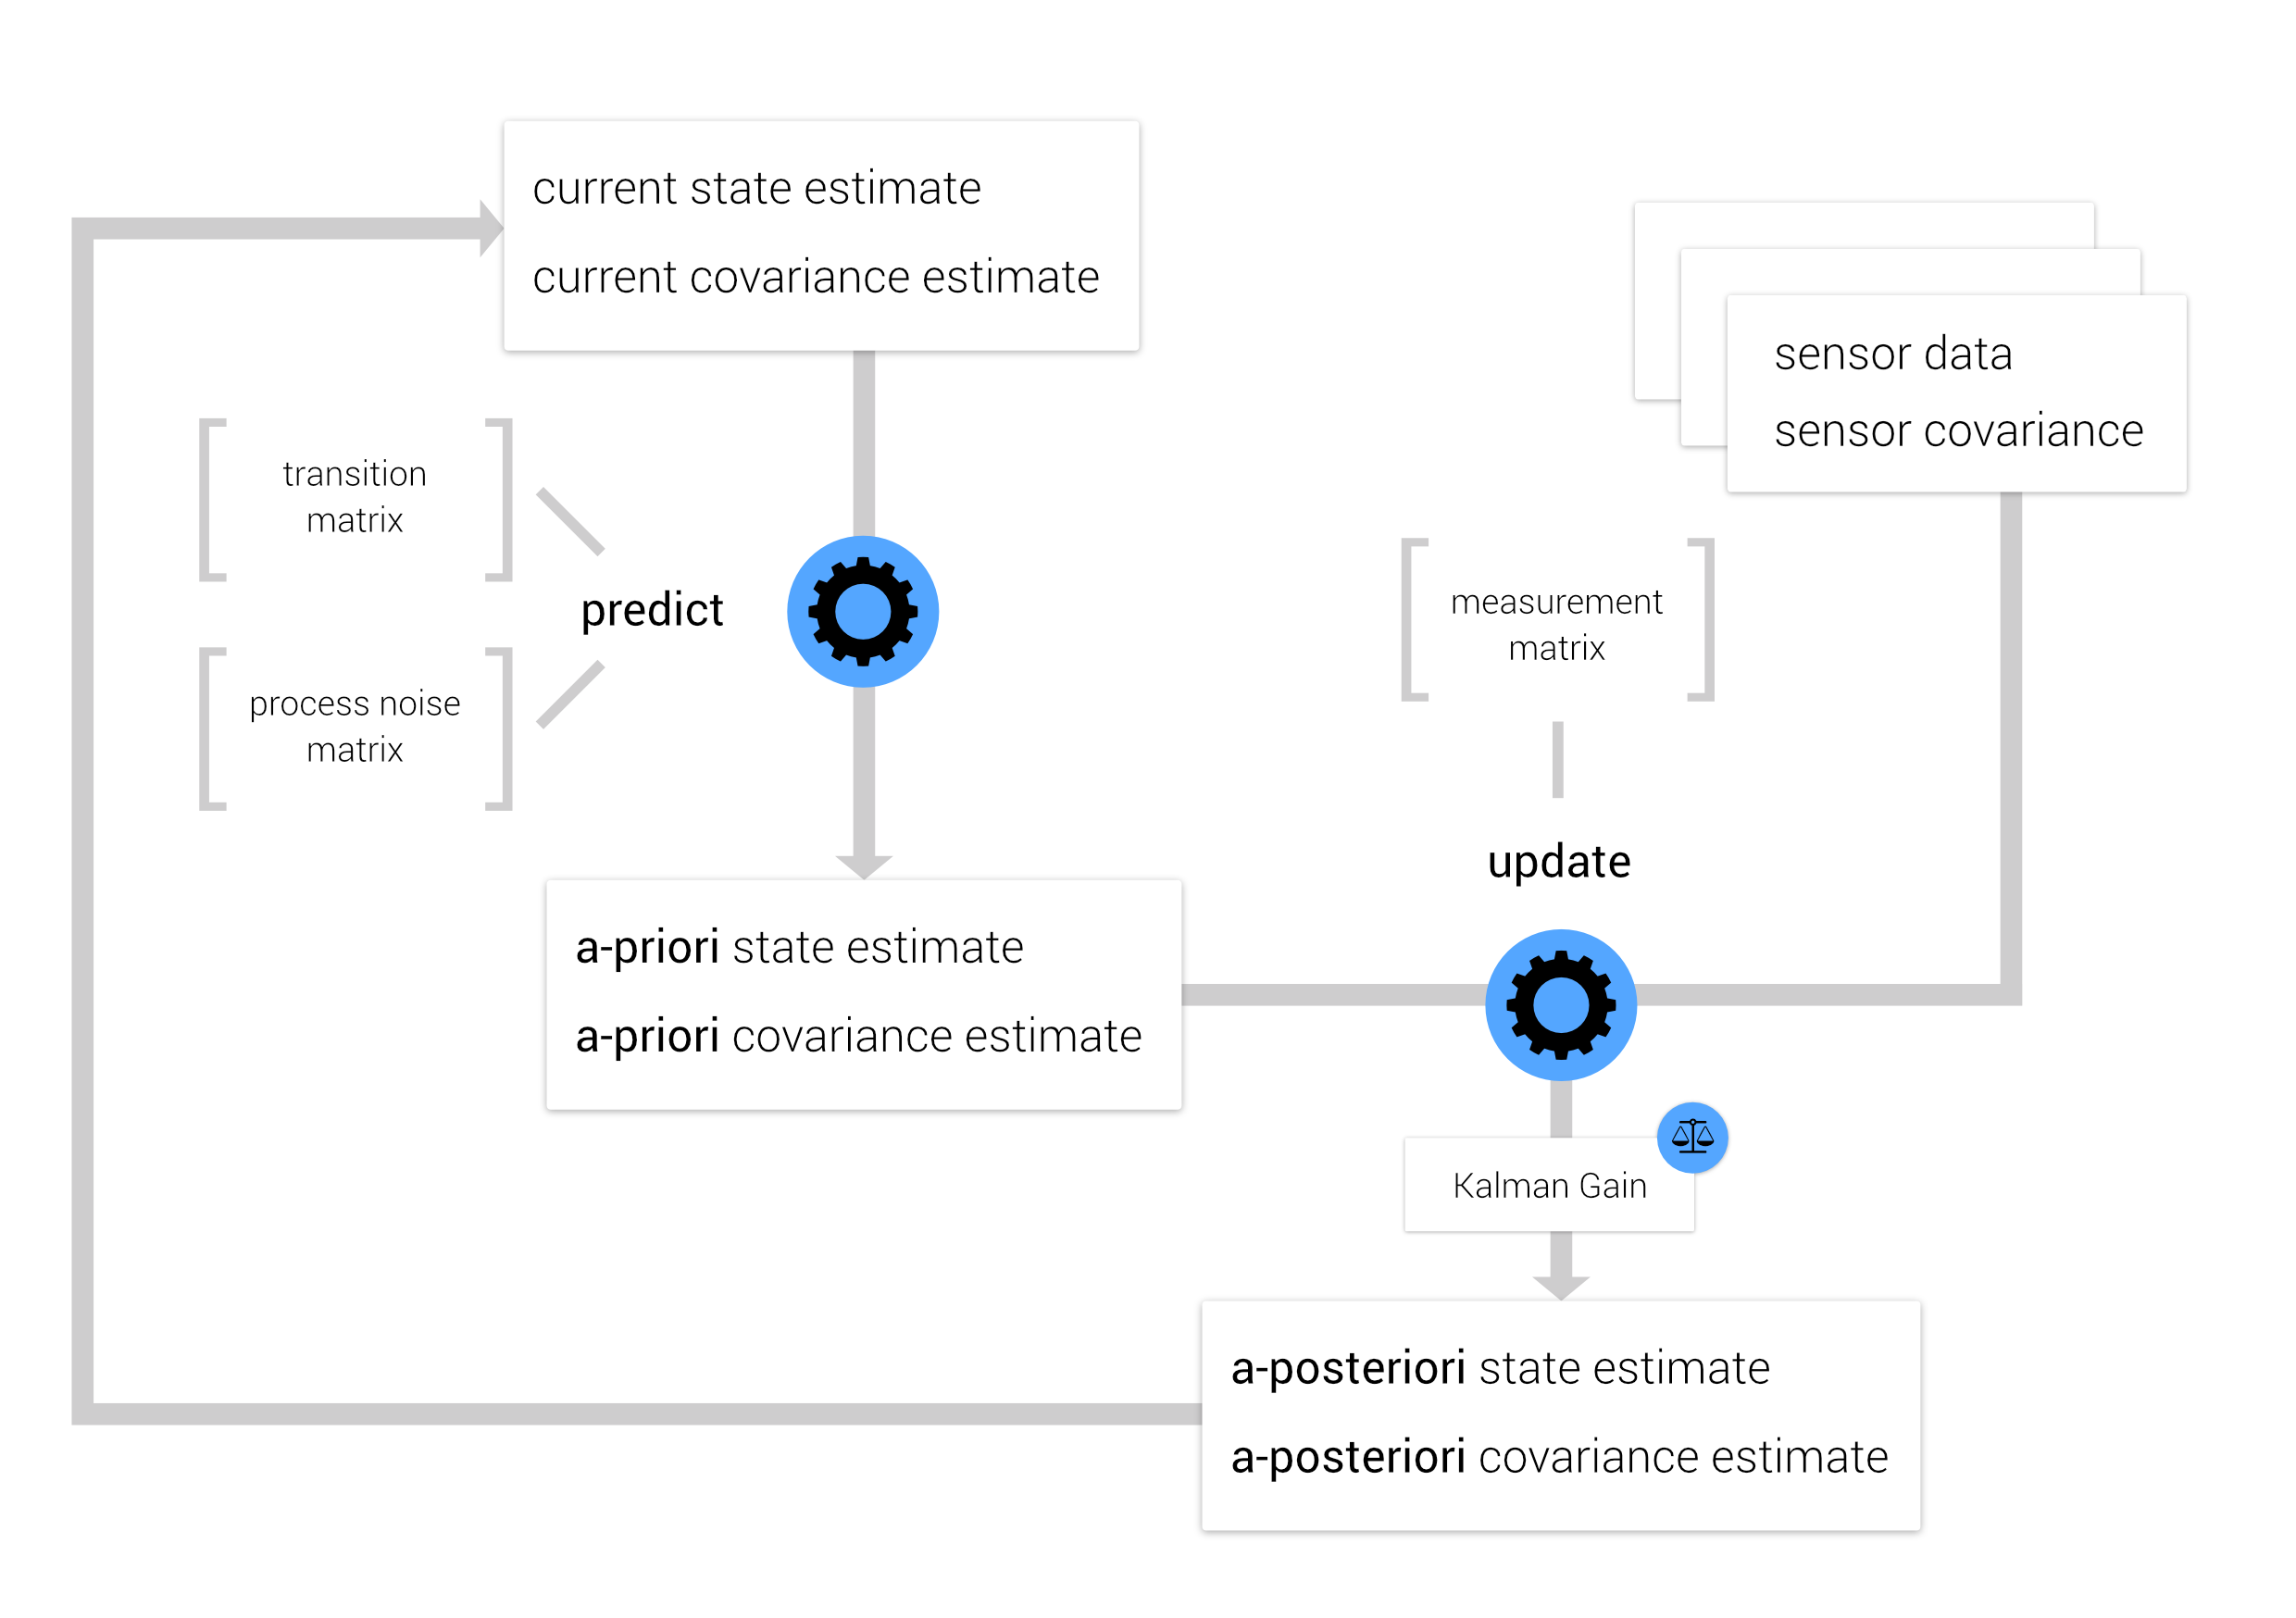
\includegraphics[width=\textwidth]{graphics/Kalman-Filter.png}
\caption{Kalman Filter overview}
\label{kalman}
\centering
\end{figure}

It can be shown that under following conditions the Kalman filter delivers optimal results, i.e. it minimizes the covariances $P$ of a state and no other linear filter produces smaller variances on the estimated error\footnote{https://www.cds.caltech.edu/~murray/wiki/images/b/b3/Stateestim.pdf, p.11-12}:

\begin{itemize}
\item The modeled process matches reality.
\item Initial state and covariance are correct.
\item there is only white (uncorrelated in time) Gaussian noise.
\item The noise's covariances are known.
\end{itemize}

